\documentclass[dvipsnames,pdf,10pt]{beamer}
\usepackage{listings,graphicx,verbatimbox,hyperref}
\usepackage{hyperref}
%\usepackage{bibentry}
% \usepackage[customcolors,shade]{hf-tikz}
% \usepackage{tikz}
\usepackage{amsmath}
\usepackage{xcolor}

\newcommand*{\colorboxed}{}
\def\colorboxed#1#{%
  \colorboxedAux{#1}%
}
\newcommand*{\colorboxedAux}[3]{%
  % #1: optional argument for color model
  % #2: color specification
  % #3: formula
  \begingroup
  \colorlet{cb@saved}{.}%
  \color#1{#2}%
  \boxed{%
    \color{cb@saved}%
    #3%
  }%
  \endgroup
}

\newcommand{\N}{\mathbb{N}}
\newcommand{\Z}{\mathbb{Z}}
\newcommand{\Q}{\mathbb{Q}}
\newcommand{\R}{\mathbb{R}}
\newcommand{\C}{\mathbb{C}}
\newcommand{\norm}[1]{\left\lVert#1\right\rVert}
\newcommand{\ceil}[1]{\lceil#1\rceil}
\newcommand{\ov}{\overline}
\newcommand{\cleq}{\preccurlyeq}
\newcommand{\cgeq}{\succcurlyeq}
\newcommand{\bdy}{\textbf{\text{Bdy}}}
\newcommand{\trace}{\text{trace}}
\newcommand{\dom}{\textbf{dom}}
\newcommand{\expec}{\mathbb{E}}
\newcommand{\bigO}{\mathcal{O}}
\newcommand{\tr}{\text{tr}}
\newcommand{\<}{\langle}
\renewcommand{\>}{\rangle}
\newcommand*\oldmacro{}%
\let\oldmacro\insertshorttitle%
% \renewcommand*\insertshorttitle{%
% \oldmacro\hfill%
% \insertframenumber\,/\,\inserttotalframenumber}
\DeclareMathOperator*{\argmax}{arg\,max}
\DeclareMathOperator*{\argmin}{arg\,min}

% use the below command to restart numbering in an enumeration, using alphabetics
% \setbeamertemplate{enumerate item}{(\alph{enumi})}
% \setbeamertemplate{enumerate subitem}{(\roman{enumii})}
\setbeamertemplate{navigation symbols}{}
\setbeamerfont{footline}{size=\fontsize{6}{10}\selectfont}
% \usetheme{Warsaw}

\usepackage[style=nature]{biblatex}
\addbibresource{refs.bib}

\DeclareCiteCommand{\footcite}[\mkbibfootnote]
  {\usebibmacro{prenote}}
  {\printnames[family-given]{labelname}%
   \hspace{1mm} \printfield{journaltitle}%
   \hspace{1mm} \printfield{year}}
  {\addsemicolon\space}
  {\usebibmacro{postnote}}

\setbeamertemplate{footline}
{
  \leavevmode%
  \hbox{%
    \begin{beamercolorbox}[wd=.25\paperwidth,ht=2.25ex,dp=1ex,center]{author in head/foot}%
      \usebeamerfont{author in head/foot}\insertshortauthor
    \end{beamercolorbox}%
    \begin{beamercolorbox}[wd=.75\paperwidth,ht=2.25ex,dp=1ex,center]{title in head/foot}%
      \usebeamerfont{title in head/foot}\insertshorttitle\hspace*{3em}
      \insertframenumber{} / \inserttotalframenumber\hspace*{1ex}
    \end{beamercolorbox}}%
  \vskip0pt%
}

\setbeamersize{text margin left=5mm,text margin right=7mm}

\usepackage{caption}
\title{Velocity gradient prediction using parameterized Lagrangian deformation models}
\author[cmhyett@math.arizona.edu]{Criston Hyett \inst{1}  \and Yifeng Tian \inst{3} \and Misha Stepanov \inst{1}  \and Daniel Livescu \inst{2}  \and Misha Chertkov\inst{1} }
\institute[shortinst]{\inst{1} Program in Applied Mathematics, University of Arizona \and
  \inst{2} CCS-2, Los Alamos National Labs \and \inst{3} CCS-3, Los Alamos National Labs}

\begin{document}
\graphicspath{{./figs/}}
%%%%%%%%%%%%%%%%%%%%%%%%%%%%%%%%%%%%%%%%%%%%%%%%%%%%%%%%%%%%%%%%%%%%%%%%%%%%% 

\begin{frame}
  \titlepage
\end{frame}

%%%%%%%%%%%%%%%%%%%%%%%%%%%%%%%%%%%%%%%%%%%%%%%%%%%%%%%%%%%%%%%%%%%%%%%%%%%%% 


%%%%%%%%%%%%%%%%%%%%%%%%%%%%%%%%%%%%%%%%%%%%%%%%%%%%%%%%%%%%%%%%%%%%%%%%%%%%% 
\begin{frame}{Summary}
  \begin{itemize}
  \item Velocity Gradient Tensor
  \item Deformation Models
  \item Baseline Model: Tensor Basis Neural Network
  \item Extending the TBNN: Parameterized Deformation Models
  \item Results
  \end{itemize}
\end{frame}
%%%%%%%%%%%%%%%%%%%%%%%%%%%%%%%%%%%%%%%%%%%%%%%%%%%%%%%%%%%%%%%%%%%%%%%%%%%%% 

%%%%%%%%%%%%%%%%%%%%%%%%%%%%%%%%%%%%%%%%%%%%%%%%%%%%%%%%%%%%%%%%%%%%%%%%%%%%% 
\begin{frame}{Velocity Gradient Tensor}
  \begin{itemize}
  \item The \textbf{velocity gradient tensor} (VGT) is defined by $A_{ij} = \frac{\partial u_i}{\partial x_j}$, so from Navier Stokes
    \begin{equation} \label{eq:NS}
      \frac{\partial u_i}{\partial t} + u_k \frac{\partial u_i}{\partial x_k} = -\frac{\partial P}{\partial x_i} + \nu \frac{\partial^2 u_i}{\partial x_k \partial x_k}
    \end{equation}

  \item We apply spatial derivatives, and use incompressibility to find the governing equations for the \textbf{Lagrangian VGT}:      
    \begin{equation}
      \frac{dA_{ij}}{dt} =
      - \colorboxed{green}{\left(A_{ik}A_{kj} - \frac{1}{3}A_{mn}A_{nm}\delta_{ij}\right)}
      - \colorboxed{red}{\left(\frac{\partial^2 P}{\partial x_i \partial x_j} -\frac{1}{3}\frac{\partial^2 P}{\partial x_k \partial x_k}\delta_{ij}\right)}
      + \colorboxed{blue}{\nu \frac{\partial^2 A_{ij}}{\partial x_k \partial x_k}}
    \end{equation}

  \item The main challenge is to predict the nonlocal \textbf{deviatoric pressure hessian} (PH), defined as
    \begin{equation}
      H_{ij} = - \colorboxed{red}{\left( \frac{\partial^2 P}{\partial x_i \partial x_j} - \frac{1}{3}\frac{\partial P}{\partial x_k \partial x_k}\delta_{ij}  \right)}
    \end{equation}
  \end{itemize}
\end{frame}
%%%%%%%%%%%%%%%%%%%%%%%%%%%%%%%%%%%%%%%%%%%%%%%%%%%%%%%%%%%%%%%%%%%%%%%%%%%%% 

%%%%%%%%%%%%%%%%%%%%%%%%%%%%%%%%%%%%%%%%%%%%%%%%%%%%%%%%%%%%%%%%%%%%%%%%%%%%% 
\begin{frame}{Lagrangian Deformation Models}
  Phenomenological ideas have tried to relate the \textbf{deformation tensor} to pressure Hessian predictions
  \begin{equation}\label{eq:Deformation-tensor}
    \frac{d D_{ij}}{dt} = A_{ik} D_{kj}, \quad \text{ with }  D_{ij}(0) = \delta_{ij},
  \end{equation}
  
  \begin{itemize}

    \only<1,3>{
    \item Chertkov et.al. used deformation in the \textbf{Tetrad Model} to resolve the finite time singularity induced by the Restricted Euler approximation to the pressure Hessian (1999)
    }

    \only<2->{
   \item Chevillard \& Meneveau, used the deformation tensor and a short-time hypothesis to create the \textbf{Recent Fluid Deformation}  model (2006)
   \item Johnson \& Meneveau enriched RFD with a better upstream condition, resulting in \textbf{Recent Deformation of Gaussian Fields} closure (2016)
   }

  \vspace{1cm}
   \only<3>{
    \item \Large{Can we \textbf{learn} what history is important?}
   }
   
 \end{itemize}

 \vspace{-1cm}
   \only<1>{
    \begin{figure}
      \centering
      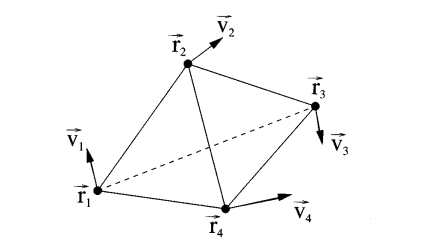
\includegraphics[width=0.5\textwidth]{tetrad.png}
      \caption{\footnotesize{Taken from Chertkov et.al. 1999 \emph{Lagrangian tetrad dynamics and the phenomenology of turbulence}}}
    \end{figure}
  }

  \only<2>{
    \begin{figure}
      \centering
      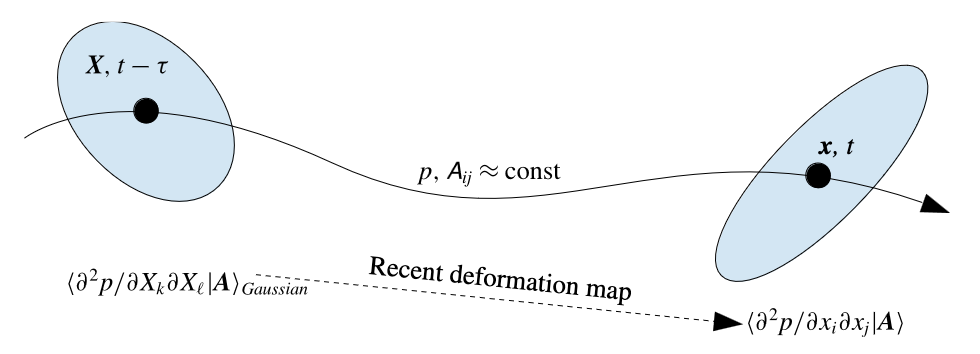
\includegraphics[width=0.6\textwidth]{recent_deformation.png}
      \caption{\footnotesize{Taken from Johnson \& Meneveau 2016 \emph{A closure for Lagrangian velocity gradient evolution in turbulence using recent-deformation mapping of initially Gaussian fields} }}
    \end{figure}
  }

 
\end{frame}
%%%%%%%%%%%%%%%%%%%%%%%%%%%%%%%%%%%%%%%%%%%%%%%%%%%%%%%%%%%%%%%%%%%%%%%%%%%%% 

%%%%%%%%%%%%%%%%%%%%%%%%%%%%%%%%%%%%%%%%%%%%%%%%%%%%%%%%%%%%%%%%%%%%%%%%%%%%% 
\begin{frame}{Baseline model: Tensor Basis Neural Network}
  Tian et.al. used physics-informed machine learning to learn a local (in time and space) closure to the PH  \begin{equation}
    \hat{H} = \sum_{i=1}^{10} g\textcolor{blue}{_{\theta}}^{(i)}(\lambda_1, \dots, \lambda_5)\cdot \hat{T}^{(i)}(\hat{A})
  \end{equation}  
  % \begin{equation*}
  %   \lambda_1 = \tr(\hat{S}^2) \quad \lambda_2 = \tr(\hat{W}^2) \quad \lambda_3 = \tr(\hat{S}^3) \quad \lambda_4 = \tr(\hat{W}^2\hat{S}) \quad \lambda_5 = \tr(\hat{W}^2\hat{S}^2)
  % \end{equation*}

  % \begin{align*}
  %   &T^{(1)} = S &T^{(2)} &= SW-WS\\
  %   &T^{(3)} = S^2 - \frac{1}{3}I \cdot \tr(S^2) &T^{(4)} &= W^2 - \frac{1}{3}I \cdot \tr(W^2)\\
  %   &T^{(5)} = WS^2 - S^2W &T^{(6)} &= W^2S + SW^2 - \frac{2}{3}I \cdot \tr(SW^2)\\
  %   &T^{(7)} = WSW^2-W^2SW &T^{(8)} &= SWS^2 - S^2WS\\
  %   &T^{(9)} = W^2S^2 + S^2W^2 - \frac{2}{3}I \cdot \tr(S^2W^2) &T^{(10)} &= WS^2W^2 - W^2S^2W
  % \end{align*}

  % \begin{itemize}
  % \item We use the natural timescale $\tau = \langle \norm{S^2}_2 \rangle^{-1}$ to normalize our VGT, and thus all of the $\lambda_i, T^{(j)}$.
  % \end{itemize}

  \begin{figure}
    \centering
    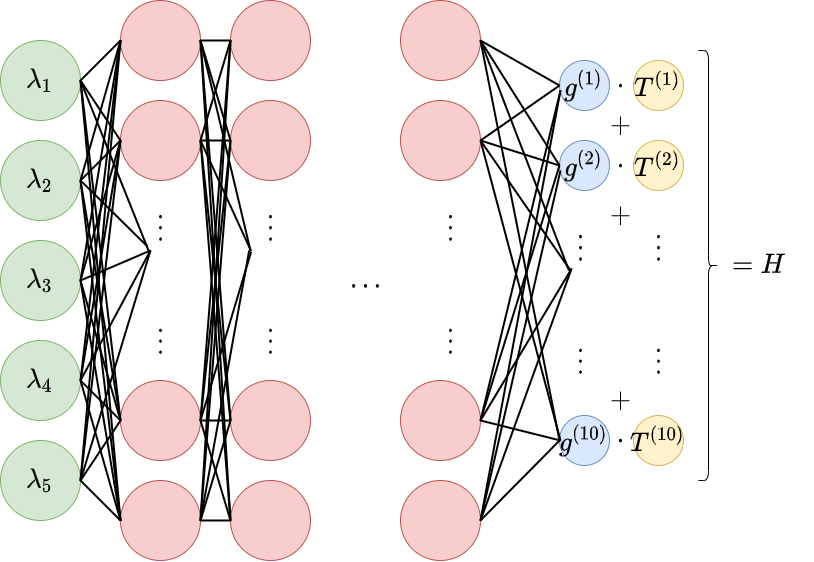
\includegraphics[width=0.6\textwidth]{tbnn.png}
  \end{figure}
  
\end{frame}
%%%%%%%%%%%%%%%%%%%%%%%%%%%%%%%%%%%%%%%%%%%%%%%%%%%%%%%%%%%%%%%%%%%%%%%%%%%%% 

%%%%%%%%%%%%%%%%%%%%%%%%%%%%%%%%%%%%%%%%%%%%%%%%%%%%%%%%%%%%%%%%%%%%%%%%%%%%% 
\begin{frame}{Parameterized Deformation Model}
  \begin{itemize}
  \item Taking the deformation tensor as inspiration, we introduce a new object,
  \begin{equation}
    X = \sum_{j = -N}^0\textcolor{blue}{\alpha_j}A(t_j)
  \end{equation}
    with $\alpha_j$ learnable parameters, and $\Delta t \approx \tau_{Kolmogorov}$

  \item We extend the TBNN using historical information via:
    \begin{equation}
      g\textcolor{blue}{_{\theta}}^{(i)}(\lambda_1, \dots, \lambda_5) \to g\textcolor{blue}{_{\theta}}^{(i)}(\lambda_1, \dots, \lambda_5, X)
    \end{equation}

    \vspace{1cm}
  \item Train and test data is \textbf{incompressible, isotropic turbulence} at \textbf{$Re \approx 240$}
    
  \end{itemize}
\end{frame}
%%%%%%%%%%%%%%%%%%%%%%%%%%%%%%%%%%%%%%%%%%%%%%%%%%%%%%%%%%%%%%%%%%%%%%%%%%%%% 


%%%%%%%%%%%%%%%%%%%%%%%%%%%%%%%%%%%%%%%%%%%%%%%%%%%%%%%%%%%%%%%%%%%%%%%%%%%%% 
\begin{frame}{Qualitative Results: $QR$ CMT}

  \begin{figure}
    \centering
    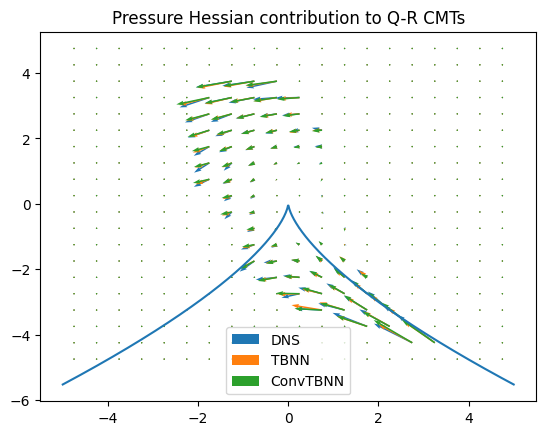
\includegraphics[width=0.8\textwidth]{qr_cmt.png}
    \caption{Qualitatively, the $QR$ conditional mean tangents match the TBNN }
  \end{figure}
\end{frame}
%%%%%%%%%%%%%%%%%%%%%%%%%%%%%%%%%%%%%%%%%%%%%%%%%%%%%%%%%%%%%%%%%%%%%%%%%%%%% 

%%%%%%%%%%%%%%%%%%%%%%%%%%%%%%%%%%%%%%%%%%%%%%%%%%%%%%%%%%%%%%%%%%%%%%%%%%%%% 
\begin{frame}{Quantitative Results: Pressure Hessian Eigenvector Alignment}
  \begin{figure}
    \centering
    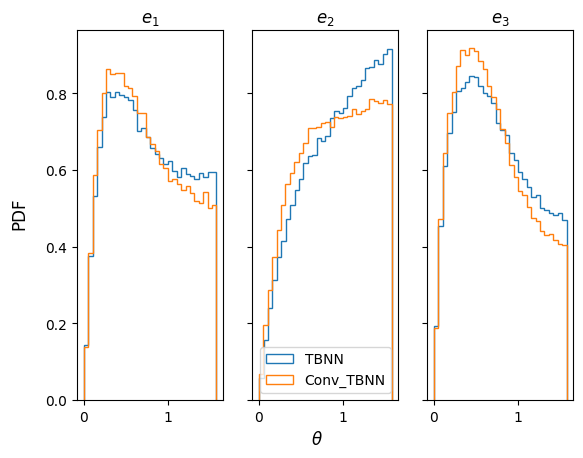
\includegraphics[width=0.7\textwidth]{eigenvector_alignment.png}
    \caption{The ConvTBNN outperforms the TBNN in eigenvector alignment}
  \end{figure}
\end{frame}
%%%%%%%%%%%%%%%%%%%%%%%%%%%%%%%%%%%%%%%%%%%%%%%%%%%%%%%%%%%%%%%%%%%%%%%%%%%%%

%%%%%%%%%%%%%%%%%%%%%%%%%%%%%%%%%%%%%%%%%%%%%%%%%%%%%%%%%%%%%%%%%%%%%%%%%%%%% 
\begin{frame}{Quantitative Results: Convolution kernel shape}

  \begin{columns}
    \column{0.4\textwidth}
    \begin{equation*}
      X = \sum_{j = -N}^0\textcolor{blue}{\alpha_j}A(t_j)
    \end{equation*}

    \column{0.6\textwidth}
    \begin{figure}
      \centering
      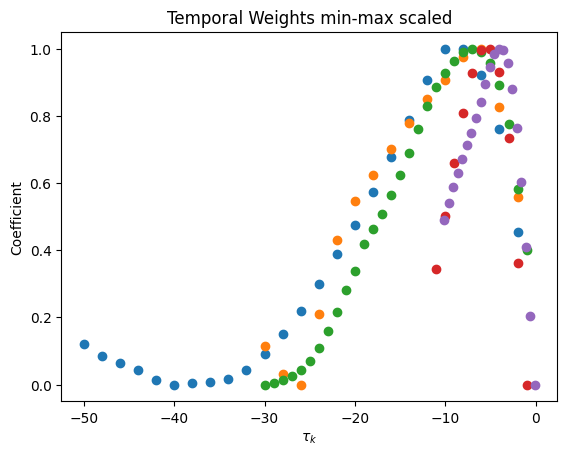
\includegraphics[width=\textwidth]{temporal_conv_kernels_minmax.png}
    \end{figure}
  \end{columns}
  \begin{enumerate}
  \item Weights are small in far history (and for short kernels no flat tails are observed)
  \item Weights are small for very recent history (redundant?)
  \item Weights in some importance region increase monotonically - reinforcing phenomenological ideas
  \end{enumerate}
\end{frame}
%%%%%%%%%%%%%%%%%%%%%%%%%%%%%%%%%%%%%%%%%%%%%%%%%%%%%%%%%%%%%%%%%%%%%%%%%%%%%


%%%%%%%%%%%%%%%%%%%%%%%%%%%%%%%%%%%%%%%%%%%%%%%%%%%%%%%%%%%%%%%%%%%%%%%%%%%%% 
\begin{frame}{Conclusion}
  \begin{itemize}
  \item By utilizing the \textbf{history of the VGT}, we can \textbf{improve the prediction of the pressure Hessian}
  \item Trained convolution kernels suggest a \textbf{finite, but significant length of important history}
  \item Can we leverage learned kernels to inform theory?
  \end{itemize}
\end{frame}
%%%%%%%%%%%%%%%%%%%%%%%%%%%%%%%%%%%%%%%%%%%%%%%%%%%%%%%%%%%%%%%%%%%%%%%%%%%%% 

%%%%%%%%%%%%%%%%%%%%%%%%%%%%%%%%%%%%%%%%%%%%%%%%%%%%%%%%%%%%%%%%%%%%%%%%%%%%% 
\begin{frame}{Parameterized Deformation Model}
  \only<1>{
  \begin{equation}\label{eq:Deformation-tensor}
    \frac{d D_{ij}}{dt} = A_{ik} D_{kj}, \quad \text{ with }  D_{ij}(0) = \delta_{ij},
  \end{equation}
  which has the formal solution
  \begin{equation}
    D(t) = \text{Texp}\left(\int\limits_0^t dt' A(t')\right) = \lim_{N\to \infty} \prod_{i = 0}^N \left( e^{A(t_i)\Delta t} \right),
  \end{equation}
  If we only take the leading order term of the discrete form:
  \begin{equation}
    D(t) \approx \left(I + \Delta t \cdot \sum_{i=0}^NA(t_i)\right)
  \end{equation}
  Taking this as motivation, we introduce a new object,
}
  \begin{equation}
    X = \sum_{j = -N}^0\textcolor{blue}{\alpha_j}A(t_j)
  \end{equation}
  \only<1>{
    and the $\alpha_j$ are learnable parameters, referred to as \textbf{convolution kernel} with $\Delta t \approx \tau_{Kolmogorov}$
  }
  \only<2>{
  \begin{itemize}
  \item We extend the TBNN using historical information via:
    \begin{equation}
      g\textcolor{blue}{_{\theta}}^{(i)}(\lambda_1, \dots, \lambda_5) \to g\textcolor{blue}{_{\theta}}^{(i)}(\lambda_1, \dots, \lambda_5, X)
    \end{equation}
  \end{itemize}
  }
\end{frame}
%%%%%%%%%%%%%%%%%%%%%%%%%%%%%%%%%%%%%%%%%%%%%%%%%%%%%%%%%%%%%%%%%%%%%%%%%%%%% 


\end{document}